\documentclass[11pt, a4paper]{article}
% \usepackage[T1]{fontenc}
\usepackage[utf8]{inputenc}
\usepackage{listings}
\usepackage[margin=1.0in]{geometry}
\usepackage{color}
\usepackage{graphicx}
\usepackage{tabularx}
\usepackage{url} 

\title{Rock the net}
\author{Elias Frantar, Samuel Schmidt, Nikolaus Schrack, Gary Ye}
\date{\today{}, Wien}
\begin{document}

\lstset{ %
  backgroundcolor=\color{white},   % choose the background color; you must add \usepackage{color} or \usepackage{xcolor}
  basicstyle=\footnotesize,        % the size of the fonts that are used for the code
  breakatwhitespace=false,         % sets if automatic breaks should only happen at whitespace
  breaklines=true,                 % sets automatic line breaking
  captionpos=b,                    % sets the caption-position to bottom
% commentstyle=\color{mygreen},    % comment style
  deletekeywords={...},            % if you want to delete keywords from the given language
  escapeinside={\%*}{*)},          % if you want to add LaTeX within your code
  extendedchars=true,              % lets you use non-ASCII characters; for 8-bits encodings only, does not work with UTF-8
% frame=single,                    % adds a frame around the code
  keepspaces=true,                 % keeps spaces in text, useful for keeping indentation of code (possibly needs columns=flexible)
% keywordstyle=\color{blue},       % keyword style
% language=bash,                   % the language of the code
  morekeywords={*,...},            % if you want to add more keywords to the set
  numbers=left,                    % where to put the line-numbers; possible values are (none, left, right)
  numbersep=5pt,                   % how far the line-numbers are from the code
  rulecolor=\color{black},         % if not set, the frame-color may be changed on line-breaks within not-black text (e.g. comments (green here))
  showspaces=false,                % show spaces everywhere adding particular underscores; it overrides 'showstringspaces'
  showstringspaces=false,          % underline spaces within strings only
  showtabs=false,                  % show tabs within strings adding particular underscores
  stepnumber=1,                    % the step between two line-numbers. If it's 1, each line will be numbered
  tabsize=2,                       % sets default tabsize to 2 spaces
  title=\lstname                   % show the filename of files included with \lstinputlisting; also try caption instead of title
}


\maketitle
\newpage
\tableofcontents
\newpage

\section{Task description}

\subsection{Basic Tasks}
Implement a simple-to-use application to monitor and configure a hardware firewall appliance “Juniper NetScreen 5GT “. The firewall allows read access over the SNMP-protocol (your app should be able to test if SNMPv3 is available and if not fallback on SNMPv2c) and write access over Telnet.
\\\\
Your app should accomplish following tasks:
\begin{itemize}
\item List all configured firewall rules (policies) on the device, add the details of the mentioned services and zones as well.
\item Allow refreshing of the list by clicking a button and by a configurable time-intervall. Your GUI should remain responsive even with short refresh-intervals!
\item Visualize the thru-put for a highlighted firewall-rule (nice2have: multiple rows) in a line-chart (configurable refresh-interval, unit bytes/sec)
\item Encapsulate the data retrieval for further reuse and easy expansion. An UML-model of your design will help you defend it at the review!
\item Build a visual appealing and easy to use interface (there is more than Swing out there).
\end{itemize} 

\subsection{Additional Tasks}
\begin{itemize}
\item Since there is only one firewall-appliance available, the time each team can test with the hardware will be strictly limited. Therefore it is essentially to use mock-objects to allow testing the app during times where the hardware is not available.
\item An additional benefit of using mock-objects will be, that a CI-Server can use them for automated building and testing.
\item You only need to consider firewall-rules for TCP and UDP connections in IPv4.
\item You can find Information about the SNMP-Mibs special for the manufacturer of the used appliance here (maybe not all of the Mibs work with the used model): 
\item http://www.oidview.com/mibs/3224/md-3224-1.html
For exploring the SNMP-Data coming from the appliance you can use tools like this:
\item http://ireasoning.com/mibbrowser.shtml
\end{itemize} 

\subsection{Advanced tasks (obligatory for grades better than B3)}
Additionally to the basic tasks your app should accomplish the following:
\begin{itemize}
\item Alarm the user visually and per email if the config of the firewall-rules changes. To avoid polling use the SNMP-trap mechanism.
\item Allow managing of firewall-rules (CRUD). To accomplish this, you will have to send configuration commands via telnet or ssh. An admin-account is available per request.
\item Use multicast-groups to build a simple transaction system to serialize administrative tasks on the firewall (for example pass an “admin token” to recognize the collaborator who is all    owed to write to the firewall). This should also work in a heterogenous environment (different implementations, different OSes), so you have to coordinate with other teams.
\item Make sure, that your interface to the firewall allows an easy change of the firewall-model (new releases, manufacturer, ...). It is not necessary to make this configurable in the GUI but must (explicitly) be considered in your software-design!
\end{itemize} 

\subsection{Teams}
Build teams with 3 to 5 participants (5 only if two or more members choose advanced level and at least one member chooses basic level). Each individual team-member has to implement, test and document code and is allowed to choose the level of difficulty he/she wants to achieve. For example: if you have a group of four students and two of them want to achieve advanced level, they can focus their implementation work on the advanced tasks. The other two team-members focus on the basic functionality. In any case there must be a working product, advanced tasks can not stand for themselves.

\subsection{Grading}
A team can apply for submission with a (mostly) functional product.
Each team-member will be graded separately, based on the documentation (and git-logs) which name him/her as author in all three main competencies as listed.
Advanced tasks will only be considered if the basic tasks are fulfilled for the most part in this team.

\subsection{Submission}
\begin{itemize}
\item Every group must have its own design/solution! Meta-group solutions will end in massive loss of points!
\item As for group work usual, a protocol with the UML-Design, the work-sharing, the timetable and test documentation is mandatory!
\item Upload your solution as a ZIP file. Please submit only the sources of your solution and a build file (build.xml, pom.xml, Makefile etc.) not the compiled class files and only approved third-party libraries. \item Your submission must compile and run!
\item Before the submission deadline, you can upload your solution as often as you like. Note that any existing submission will be replaced by uploading a new one.
\end{itemize}

\newpage

\section{Effort estimation}
\subsection{Basic Tasks}
\begin{tabular} {| l | c | c | c |} \hline
Task &	Original Estimate & Remaining Estimate & Time spent \\ \hline
Preparation for the Tasks &	20 &	0.00 & 24.50 \\ \hline
Listing firewall rules &	7 &	2 &	9.50 \\ \hline
Refreshing rules &	6 &	6 &	0.00 \\ \hline
Visualize thru put & 8 &	4 &	5.00 \\ \hline
Encapsulate the data retrieval &	4	& 0.00 &	4.00 \\ \hline
GUI	 & 10 &	7 &	8.00 \\ \hline
Final Documentation  &	8	& 2	& 5.00 \\ \hline
Basic Total	& 63 &	31.00 &	56.00 \\ \hline
\end{tabular}
\subsection{Advanced Tasks}
\begin{tabular} {| l | c | c | c |}\hline
Task &	Original Estimate & Remaining Estimate & Time spent \\ \hline
Alarm the user &	7	& 5	& 0 \\ \hline
Firewall rules CRUD &	6 &	8 & 	0 \\ \hline
Transactions by Multicast &	8 &	15 &	0 \\ \hline
Exchangeable & 5 & 0	 & 2 \\ \hline
Advanced Total & 26 &	28 &	2 \\ \hline
\end{tabular}

\subsection{Total}
\begin{tabular} {| l | c | c | c |}\hline
	Task &	Original Estimate & Remaining Estimate & Time spent \\ \hline
	Total & 89 & 31 & 58 \\ \hline
\end{tabular}

\section{Design}
\subsection{User Stories}
 \textbf{Basic tasks:}
\begin{itemize}
\item As a user, I want to connect to my firewall device by entering its IP-address.
\begin{itemize}
\item As a user, I want to connect with SNMPv3.
\item As a user, I want to fallback to SNMPv2c when SNMPv3 is not available.
\end{itemize}
\item As a user, I want a visually appealing graphical user interface.
\item As a user, I want to list all firewall-rules configured on my device.
\begin{itemize}
\item As a user, I want to see the port of a firewall rule.
\item As a user, I want to see the zone of a firewall rule.
\item As a user, I want to see the service of a firewall rule.
\item As a user, I only want to see the TCP and UDP firewall rules.
\end{itemize}
\item As a user, I want the rules to be refreshed.
\begin{itemize}
\item As a user, I want the rules to be refreshed automatically.
\begin{itemize}
\item As a user, I want to configure the refresh intervals.
\end{itemize}
\item As a user, I want to refresh the rules manually by pressing on a button.
\end{itemize}
\item As a user, I want to visually monitor the thru-put of a firewall-rules.
\begin{itemize}
\item As a user, I want to visually see the thru-put in line-chart.
\item As a user, I want to monitor multiple rules at the same time.
\end{itemize}
\item As a developer, I want the data retrieval to be encapsulated for further reuse and expansion.
\item As a developer, I want all network packages to be logged in a log file for debugging purposes.
\end{itemize}
 \textbf{Advanced tasks:}
\begin{itemize}
\item As a user, I want to be notified if a rule has been changed without my assistance.
\begin{itemize}
\item As a user, I want to be notified by a pop-up window.
\item As a user, I want to be optionally notified by email.
\item As a user, I want to configure my email-address.
\begin{itemize}
\item As a user, I want to configure the email-address in a config-file.
\item As a user, I want to configure the email-address in the GUI.
\end{itemize}
\end{itemize}
\item As a user, I want to configure all firewall-rules on the device.
\begin{itemize}
\item As a user, I want to create a fully new rule.
\item As a user, I want to fully edit an existing rule.
\item As a user, I want to delete an existing rule.
\item As a user, I want to login before editing a rule.
\begin{itemize}
\item As a user, I want to stay logged in for the whole session after I have logged in for the first time.
\end{itemize}
\end{itemize}
\item As a user, I want to have a transaction system for write access on the firewall, so that no editing conflicts can occur when multiple applications are trying to modify at the same time.
\item As a developer, I want to be able to easily modify the software so that it works with other firewall hardwares.
\begin{itemize}
\item As a developer, I only want to exchange the SNMP-commands to make the application work with other firewall hardwares.
\end{itemize}
\end{itemize}

\subsection{Basic}
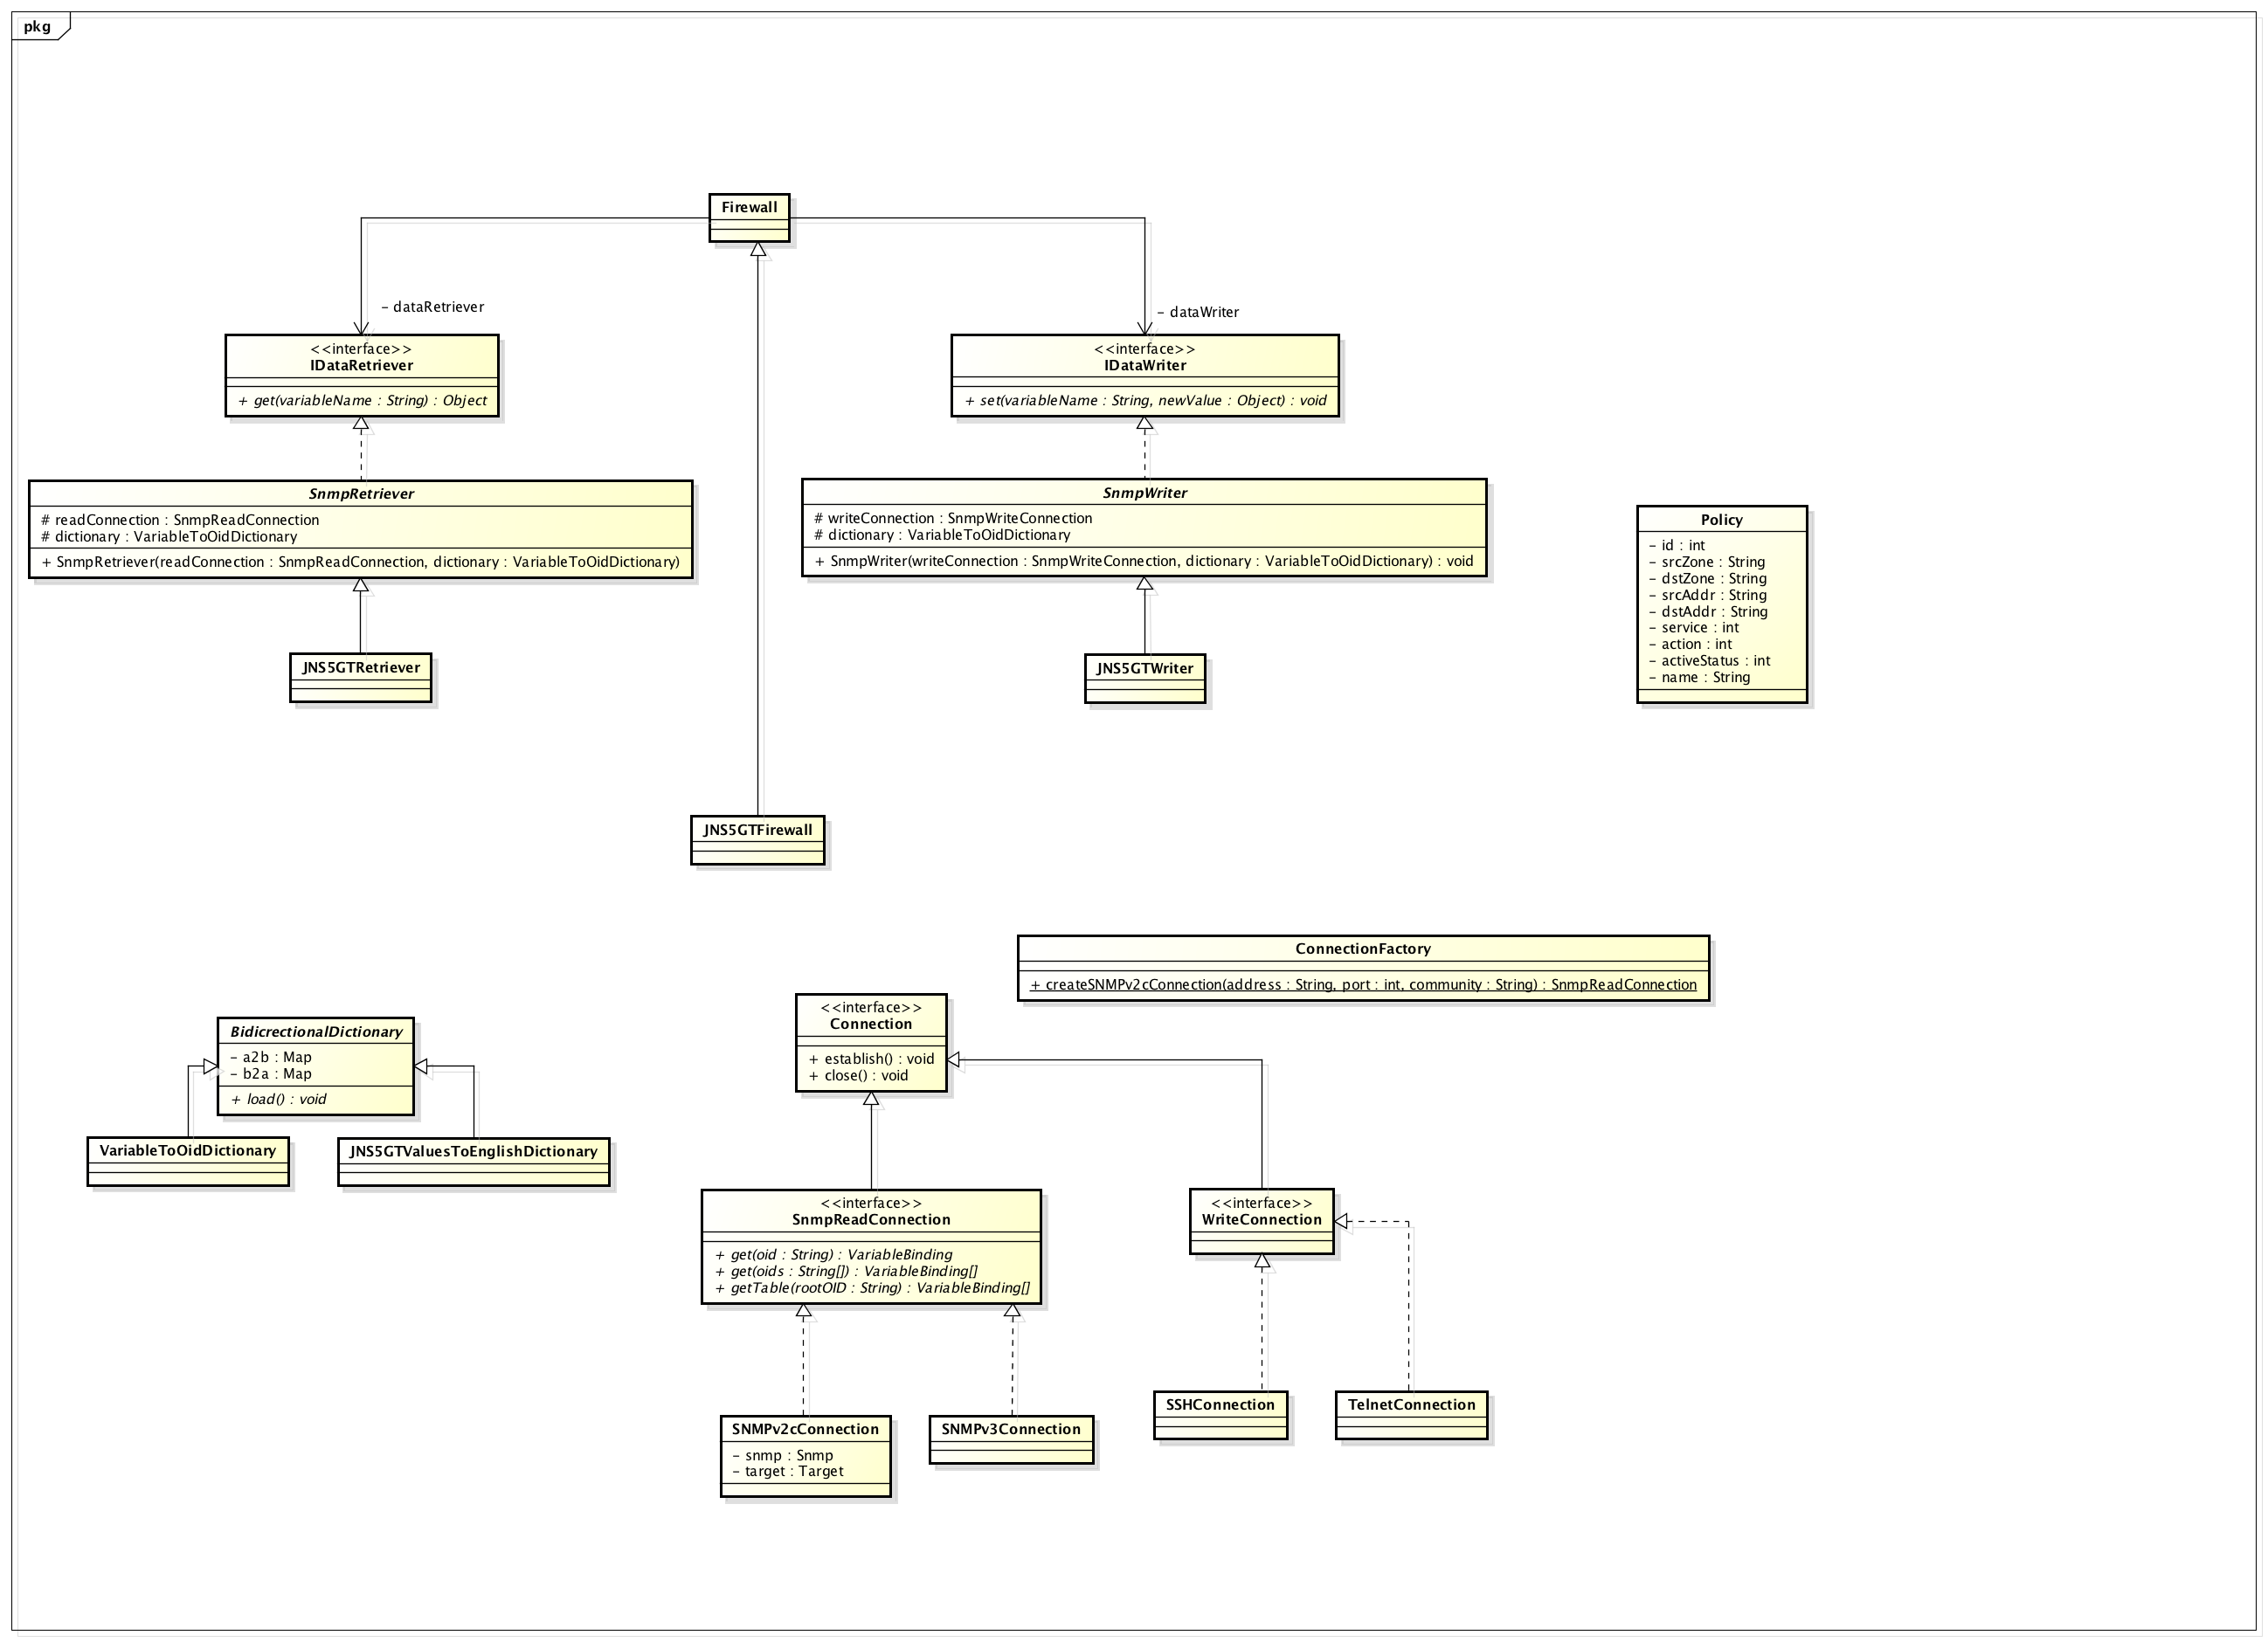
\includegraphics[width=\textwidth]{images/uml}

% add the next one

\section{Installation and Preparation}

\section{Technologies}
\subsection{Mock-Objects}
\subsubsection{Setup}

\begin{enumerate}
	\item Download \textit{Mockito} from \cite{MockitoDownload}
	\item Add \textit{junit-4.11.jar} and \textit{mockito-all-1.9.5.jar} to the project's \textit{classpath}
	\item Done
\end{enumerate}

\subsubsection{How to use Mockito}

\textit{Mockito} allows you to mock interfaces, but also concrete classes, with a single line of code:
	
\begin{lstlisting} 
List mockedList = mock(List.class); // creates a mock-Object of `List` 
\end{lstlisting}
	
A \textit{Mockito-Mock-Objects} remembers all methods, which have been called. So you can check afterwards if some method has been called with some parameters.
	
\begin{lstlisting}
	mockedList.add("one");
	    
	verify(mockedList).add("one"); // test "successful" because that exact method with that exact parameter has been called before
	verify(mockedList).add("two"); // test "failed" because `.add("two")` has not been called before
\end{lstlisting}

One of the main functionalities of a Mock-object is that it can provide kind of dummy-methods, called *stubs*, i.e. when a specific method with a specific parameter is called, a specific
value is returned. There are also some kind of wildcards for the methods parameters, if you want to return "first" on any given Integer-parameter. That can be achieved like this:

\begin{lstlisting}
    when(mockedList.get(0)).thenReturn("first"); // `mockedList` will return "first" when `.get(0)` is called
    System.out.println(mockedList.get(0)); // prints "first"
    
    when(mockedList.get(anyInt()).thenReturn("any int"); // will return "any int" if you pass for example: 1, 27, 4, ...
    System.out.println(mockedList.get(2345)); // prints "any int"
\end{lstlisting}

You can also make the mock throw Exceptions by using `.thenThrow()` or make void methods throw Exceptions by:

\begin{lstlisting}
    doThrow(new RuntimeException()).when(mockedList).clear();
    mockedList.clear(); // throws RunTime-Exception
\end{lstlisting}

You can also verify how often a specific method has been called. That works like this:

\begin{lstlisting}
    mockedList.add("once");
    
    verify(mockedList, times(1)).add("once"); // success because `.add("once")` has been called exactly once
    verify(mockedList, times(2)).add("once"); // fails because it has only been called once
\end{lstlisting}

For \textit{times(0)}, you should better use \textit{never()}.
 
Like the number of invocations, you can also verify the order of of invocations:

\begin{lstlisting}
    mockedList.add("first");
    mockedList.add("second");
    
    InOrder inOrder = inOrder(mockedList);
    
    inOrder.verify(mockedList).add("first");
    inOrder.verify(mockedList).add("second");  
\end{lstlisting} 
    
For explanation of additional functionalities and full documentation, see \cite{MockitoDownload}.

\subsection{Java FX}
Java 8 supports Java FX, so no further installation will be needed if Java 8 is used. 

\subsubsection{Line Charts}

For the application a line chart has been needed. Using the LineChart class it is possible to show up a pretty visual appealing line chart which updates with or without animation.

A sample picture of the Java FX LineChart is shown below. 

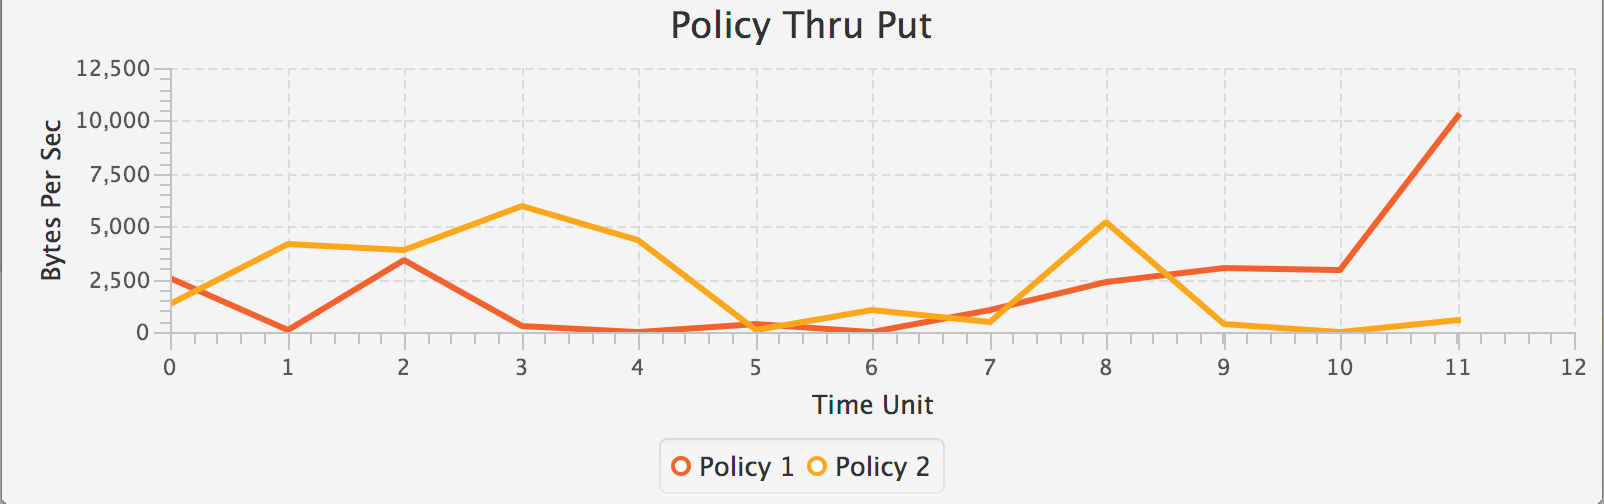
\includegraphics[width=\textwidth]{images/linechart.png}

% http://docs.oracle.com/javafx/2/charts/line-chart.htm#CIHGBCFI

\subsection{SNMP - Simple Network Management Protocol}

It is, like the name says, a simple network protocol to manage and monitor the devices in a network. Practically, the monitored devices are all connected to a central system that controls them by using the “Simple Network Manager Protocol”.

\begin{figure}[h!]
	\centering
	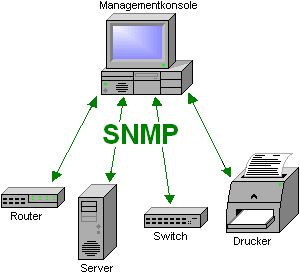
\includegraphics[width=0.6\textwidth]{images/SNMP-Managementkonsole.png}
	\caption{The Router, the Server, the Switch and the Printer are connected via the SNMP to the management system.}
\end{figure}


% (Source: http://de.wikipedia.org/wiki/Simple_Network_Management_Protocol)

\subsubsection{SNMPv2c and SNMPv3 differences}

With v3 no changes to the protocol aside from added security and remote configuration enhancements to SNMP were added. However new textual conventions, concepts and terminology were introduced.

The core Snmp class documentation \cite{SNMP4JDoc} offers only insight on big differences in SNMPv1(asynchronous) and v3(synchronous) implementations. TransportMapping only affects UDP/TCP/… configurations.

\subsection{MIB - Management Information Base}
As the management system wants to read data from a device, it has to know how the structure of the data storage. The specified informations can be retrieved from the corresponding MIB. 

The MIB of the device, that is being used for this exercise, can be found from \cite{MIBDownload}.

The MIB is structured like a tree (examples can be found in the Wikipedia article). Every object of the device can be identified by the OID (Object Identifier), which is just a list of numbers separated by a dot.

One can for example GET/SET the variables by using the OI of the specified object.

Also one can use a MIB browser to explore the structure \cite{MIBBrowser}.
\subsection{Multicast-Groups}

Multicast is basically a group communication where the packages are sent only once and arrive at their destination simultaneously. The nodes of the network (router, switches) will take care of how the messages will be distributed. So the sender does not have to worry about the number of receivers.

The most common protocol for this is UDP, even though it’s unreliable. There exists also reliable protocols where loss detection and retransmission are provided.

In the Java API there exists a class which provides multicasting \cite{javamulticast}. The documentation itself says:
“A multicast group is specified by a class D IP address and by a standard UDP port number. Class D IP addresses are in the range 224.0.0.0 to 239.255.255.255, inclusive. The address 224.0.0.0 is reserved and should not be used.”

A code snippet has also been provided:

\begin{lstlisting}
// join a Multicast group and send the group salutations
...
String msg = "Hello";
InetAddress group = InetAddress.getByName("228.5.6.7");
MulticastSocket s = new MulticastSocket(6789);
s.joinGroup(group);
DatagramPacket hi = new DatagramPacket(msg.getBytes(), msg.length(),
group, 6789);
s.send(hi);
// get their responses!
byte[] buf = new byte[1000];
DatagramPacket recv = new DatagramPacket(buf, buf.length);
s.receive(recv);
...
// OK, I'm done talking - leave the group...
s.leaveGroup(group);
\end{lstlisting}

The important methods of the MulticastSocket class are:
\begin{description}
\item[joinGroup] to join the given group
\item[receive] receive the message of the subscribed group
\item[leaveGroup] leave the specified group
\end{description}

\section{Test report}
\section{Occurred problems}

\nocite{*}
\bibliographystyle{plain}
\bibliography{bibliography}{}

\end{document}
